\chapter{Opis bazy mobilnej}

\section{Dookólna baza jezdna}

Bazą sprzętową, wykorzystywaną w niniejszej praca jest dookólna baza mobilna. Jest to baza holonomiczna, która może poruszać się w dowolnym kierunku bez zmiany swojej orientacji oraz zmienić kierunek ruchu w dowolnej chwili. Możliwe jest to dzięki zastosowaniu kół szwedzkich. Koła te umieszczone są w narożnikach prostokątnej platformy i napędzane są niezależnie przez serwomotory. Dzięki zamontowanym enkoderom możliwy jest odczyt z odometrii robota. Platformę przedstawia rysunek [\ref{fig:omnivelma}]. \\

\begin{figure}[H]
	\centering
	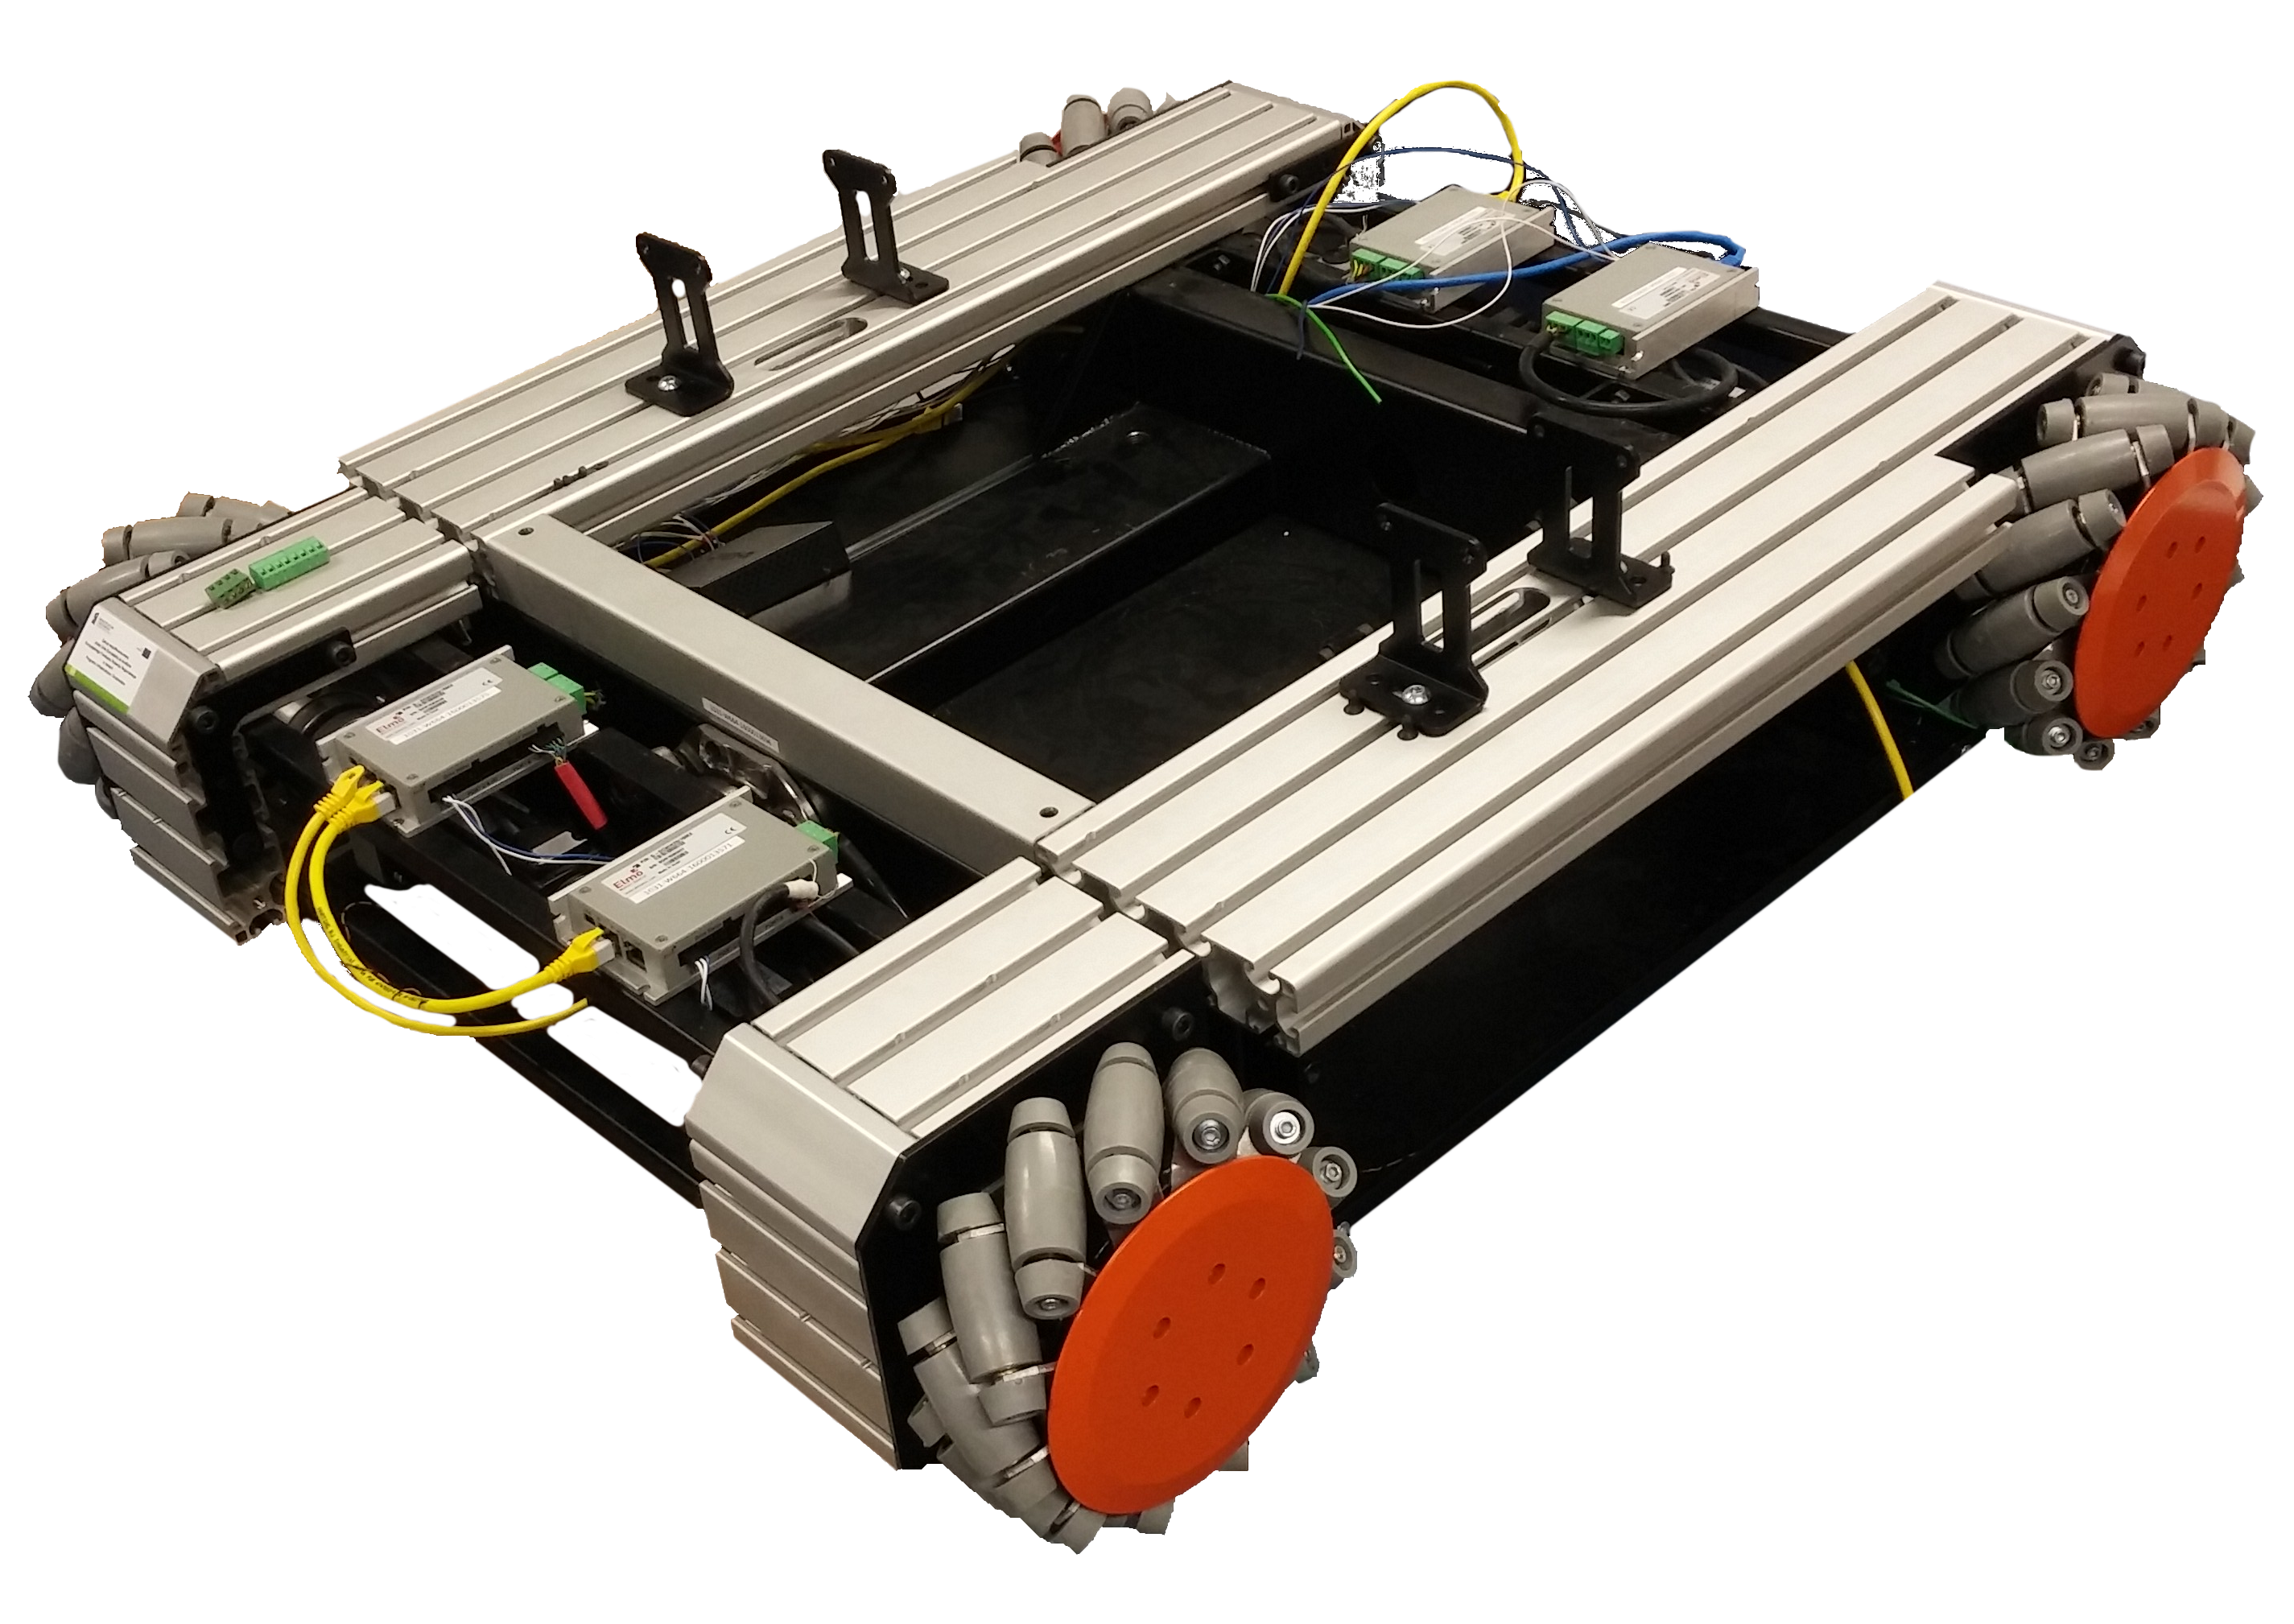
\includegraphics[width=0.55\textwidth]{gfx/omnivelma.png}
	\caption{Dookólna baza mobilna \cite{omnivelma}}
	\label{fig:omnivelma}
\end{figure}

Koła szwedzkie mają specjalne rolki ustawione pod kątem $45^{\circ}$ w stosunku do osi obrotu koła. Rolki te są pasywne, podążają jedynie za ruchem koła macierzystego. Ustawienie globalne kół, w znaczeniu kierunku skierowania rolek na platformie odpowiada literze $X$, patrząc na platformę z góry. W kole szwedzkim wyróżnia się dwa kierunki ruchu: ruch napędzany w kierunku równoległym do płaszczyzny koła oraz ruch swobodny w kierunku prostopadłym do osi obrotu rolki będącej aktualnie w kontakcie z podłożem. Ustawienie to dostrzec można na rysunku [\ref{fig:omnivelma}]. Szkic kół szwedzkich pokazano na rysunku [\ref{fig:wheels}].

\begin{figure}[H]
	\centering
	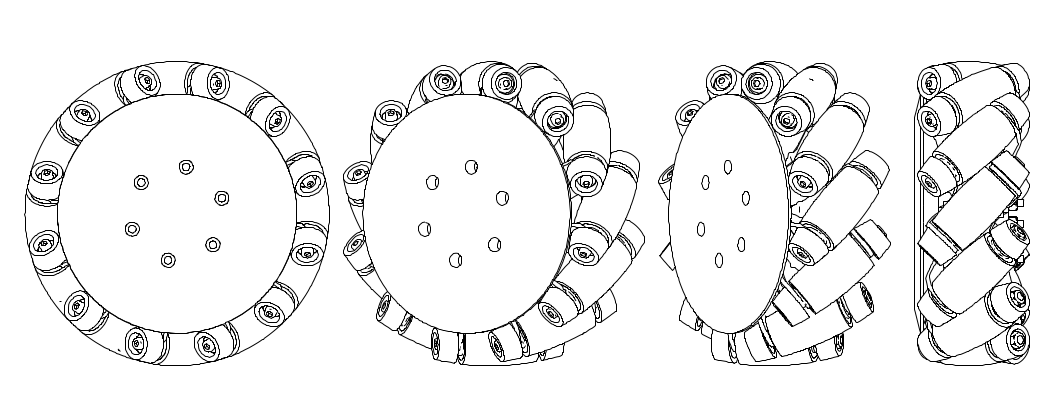
\includegraphics[width=0.5\textwidth]{gfx/wheels.png}
	\caption{Koła szwedzkie \cite{omnivelma}}
	\label{fig:wheels}
\end{figure}

Ruch platformy odbywa się poprzez odpowiednie zadawanie prędkości każdego z kół. Konstrukcja koła szwedzkiego powoduje, że nie występuję tarcie w kierunku $45^{\circ}$ do osi obrotu koła. Ma to istotne znaczenie, gdyż siła jaka działa na koło jest prostopadła do tego kierunku (moment siły jest równoległy do osi koła). Konstrukcyjnie więc ustawiając koła w literę $X$ i odpowiednio manipulując wartościami prędkości dla każdego z kół, otrzymujemy możliwość ruchu w dowolnym kierunku. Momenty sił, siły, wektory prędkości kół oraz kierunek poruszania się platformy demonstruję rysunek [\ref{fig:vectors}].

\begin{figure}[H]
	\centering
	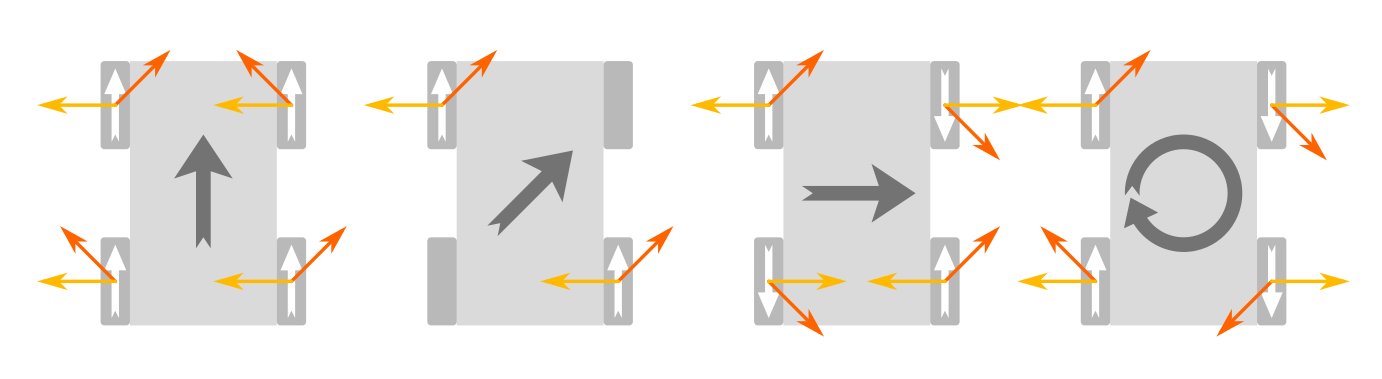
\includegraphics[width=0.9\textwidth]{gfx/vectors.png}
	\caption{Ruch platformy mobilnej (widok z góry) - ciemna strzałka symbolizuję kierunek ruchu platformy, biała ruch koła, strzałka żółta to moment siły działający na dane koło, a czerwono-pomarańczowa to kierunek siły działającej na to koło \cite{omnivelma}}
	\label{fig:vectors}
\end{figure}

Ruch platformy można opisać równaniem \eqref{eq:kinematic} kinematyki prostej:

\begin{equation} \label{eq:kinematic}
	\begin{bmatrix}
	v_x \\
	v_y \\
	\omega_z \\
	\end{bmatrix}
	=
	\frac{r}{4}
	\begin{bmatrix}
	-1 & 1 & -1 & 1 \\
	1 & 1 & 1 & 1 \\
	\frac{2}{a+b} & \frac{-2}{a+b} & \frac{-2}{a+b} & \frac{2}{a+b} \\
	\end{bmatrix}
	\begin{bmatrix}
	\omega_1 \\
	\omega_2 \\
	\omega_3 \\
	\omega_4 \\
	\end{bmatrix}
\end{equation} 

Zmienne $v_{x}, v_{y}$ wykorzystane w równaniu to zadane prędkości liniowe, $w_{z}$ to prędkość kątowa platformy wokół osi z, $r$ jest promieniem koła, $a$ to rozstaw kół na tej samej osi, $b$ to rozstaw osi. Zmienne $w_{i}$ to prędkość kątowa koła. Numerację kół przedstawia rysunek [\ref{fig:n}]
  	 
\begin{figure}[H]
  	\centering
  	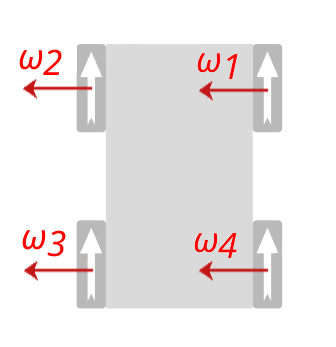
\includegraphics[height=4cm]{gfx/vectors2.png}
    \caption{Numeracja kół platformy dookólnej}
    \label{fig:n}
\end{figure}
        

Użycie platformy dookólnej ma uzasadnienie w kontekście realizacji ruchu w środowisku pracy z człowiekiem, ponieważ pozwala na efektywne tworzenie ścieżki ruchu, bez narzutu ograniczeń ruchu bazy nieholonicznej. Przy bardzo bliskiej detekcji człowieka, bądź jego względnie dużej prędkości, system nie byłby w stanie stworzyć odpowiedniej trajektorii dla robota, co mogłoby powodać zatrzymanie ruchu do czasu oddalenie się osoby. Ponad to platforma dookólna sprawnie porusza się w wąskich przejściach oraz potrafi obrócić się w miejscu. \\


\section{Czujniki}

\subsection{Kinect}

Kinect jest czujnikiem wyprodukowanym przez Microsoft dla konsoli Xbox 360 \cite{kinect2}. W oryginalnym zastosowaniu czujnik był wykorzystywany do obsługi konsoli za pomocą gestów i poleceń głosowych oraz wykorzystany był w grach wideo. Jest również często wykorzystywany w robotyce ze względu możliwości i niską cenę. Urządzenie składa się z promiennika podczerwieni oraz dwóch kamer - kamery wizyjnej RGB oraz kamery na podczerwień (IR) zwracającej informację o głębi obrazu. Emiter podczerwieni emituję wiązkę promieni podczerwonych, a kamera podczerwieni bada odbicia promieni od obiektów. Im obiekt jest bliżej, tym mocniejsze pada na niego światło. W ten sposób otrzymuję się chmurę punktów, reprezentującą rozmieszczenie przestrzenne obiektów i interpolowany obraz głębi \cite{kinect}.

\begin{figure}[H]
	\centering
	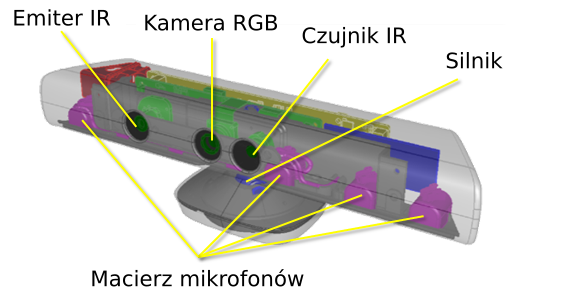
\includegraphics[width=0.8\textwidth]{gfx/kinect2pl.png}
	\caption{Budowa Kinecta - emiter podczerwieni, kamera RGB, czujnik głębi, silnik i macierz mikrofonów \cite{kinect}}
	\label{fig:kinect}
\end{figure}

Kinect zawiera również macierz mikrofonów, pozwalającą na realizację wykrywania komend użytkownika oraz silnik pozwalający na zmianę kąta pochylenia bazy. Tabela [\ref{tab:kinect_specification}] przedstawia specyfikacje urządzenia.

\begin{table}[H]
\centering
{\renewcommand{\arraystretch}{1.5}
\begin{tabular}{ p{5cm} | p{7cm} }
 Rozdzielczość obrazu RGB & 640x480 \\
 \hline
 Rozdzielczość obrazu głębi (interpolowana) & 300x200 (640x480) \\
 \hline
 Zakres pracy & 0.4m-6.5m \\
 \hline
 Pole widzenia & $43^{\circ}$ pionowo, $57^{\circ}$ poziomo \\
 \hline
 Klatki na sekunde (dla obu kamer) & 30 \\
 \hline
 Format audio & 16-kHz, 24-bit, modulacja PCM \\
 \hline
 Charakterystyka audio & Macierz czterech mikrofonów 24-bit, przetwornik A/C, niwelacja echa i szumu
\end{tabular}}
\caption{Specyfikacja czujnika Kinect \cite{kinect}}
\label{tab:kinect_specification}
\end{table}

Posługująć się inżynierią wsteczną ustalono, że Kinect jest w stanie dostarczyć obraz RGB o rozdzielczości do 1280x1024, lecz przy zmniejszonej liczbie klatek na sekundę. Wysyła on także bezpośrednio (zanim zostanie skonwertowany na mapę głębi) obraz z kamery IR w rozdzielczości 640x480, lub 1280x1024 przy zmniejszeniu liczby klatek na sekundę. Rzeczywisty zakres pracy określono na 1.2m-3.5m \cite{kinect_openkinect}. \\

Obraz RGB oraz dane o błębokości obrazu posłużą do wykrycia i ustalenia orientacji człowieka w przestrzeni. Baza mobilna sama w sobie nie posiada jednak zamontowanego Kinecta, co będzie poruszane w trakcie implementacji.\\

\subsection{LIDAR}

Zasada działania skanerów laserowych LIDAR opiera się na wysyłaniu wiązki laserowej i mierzenia czasu jej powrotu po odbiciu od obiektów. Na tej podstawie otrzymuję się informację o rozmieszczeniu obiektów w polu widzenia sensora. Wewnątrz sensora znajduje się ustawione pod kątem $45^{\circ}$ w stosunku do pionu lustro. Lustro zamontowane jest na wale silnika wraz z enkoderem. Urządzenie emituje wiązkę laserową i na podstawie opóźnień w czasie powrotu wiązki do detektora oraz kąta obrotu wału silnika generowane są wyniki pomiarów \cite{lidar}. 


\begin{figure}[H]
	\centering
	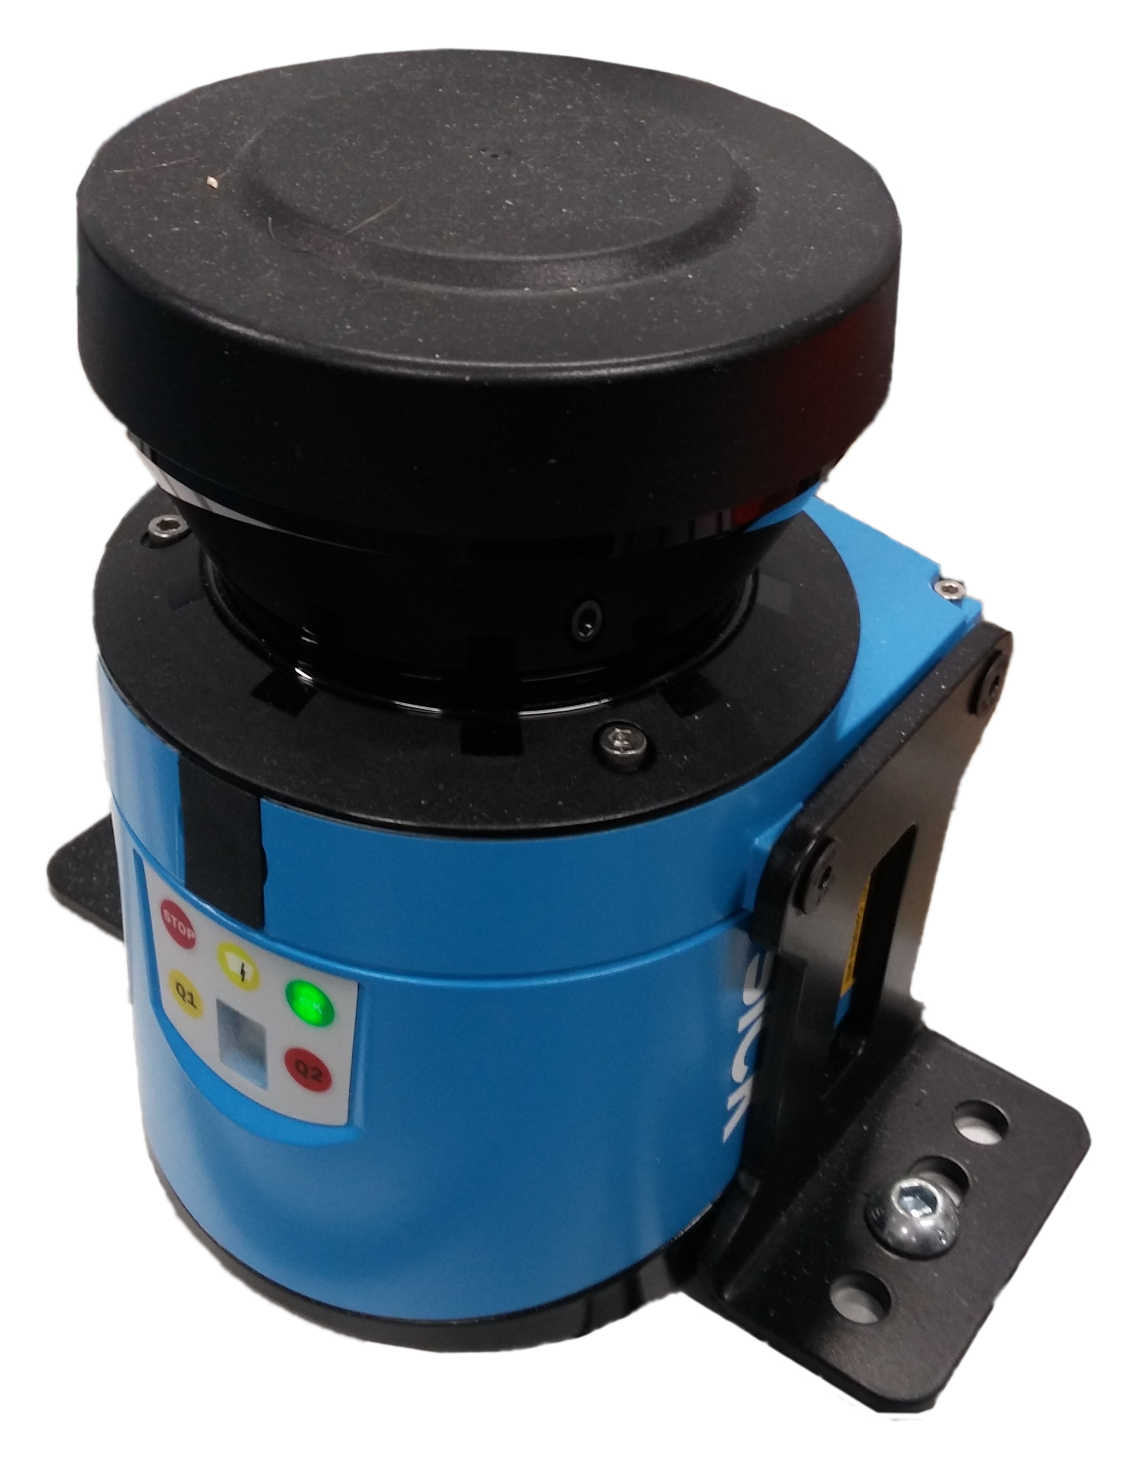
\includegraphics[width=0.33\textwidth]{gfx/lidar.png}
	\caption{LIDAR LMS100-1000 firmy SICK}
	\label{fig:sick}
\end{figure}


Platforma mobilna wyposażona jest w dwa czujniki LIDAR LMS100-1000 firmy SICK (rysunek \ref{fig:sick}). Umiejscowione po jej przeciwnych stronach. Powodem zastosowania dwóch skanerów jest ograniczone pole widzenia pojedynczego czujnika. Dwa skanery pozwalają dookólną obserwację otoczenia. Specyfikację techniczą skanera przedstawia tabela [\ref{tab:lidar_specification}].

\begin{table}[H]
\centering
{\renewcommand{\arraystretch}{1.5}
\begin{tabular}{ p{8cm} | p{4cm} }
 Pole widzenia & $270^{\circ}$\\
 \hline
 Długość wykorzystanej fali lasera & 905nm (podczerwień) \\
 \hline
 Częstotliwość pracy & 50Hz \\
 \hline
 Maksymalna odległość pomiaru & 20m \\
 \hline
 Rozdzielczość pomiaru & $0.5^{\circ}$ \\
 \hline
 Systematyczny błąd pomiarowy & 0.03m \\
 \hline
 Przypadkowy błąd pomiaru odległości & 0.012m \\
\end{tabular}}
\caption{Specyfikacja skanera laserowego LIDAR LMS100-1000 firmy SICK \cite{omnivelma}}
\label{tab:lidar_specification}
\end{table}


Skanery LIDAR w niniejszej pracy są wykorzystywane do tworzenia mapy środowiska, wykrywania przeszkód oraz detekcji człowieka.